\documentclass{beamer}

%%%% Packages
\usepackage{amsmath, amsthm, amssymb}
%% \usepackage[english]{babel}
\usepackage{array}              % for >{} in table column
% specification
\usepackage{color}              % for color definition
\usepackage{colortbl}
\usepackage{graphicx}
\usepackage{multirow}           % for multirow
\usepackage{multicol}           % for multiple columns
\usepackage{tabularx}           % for centering in table
\usepackage{tikz}               % for drawing diagrams
\usetikzlibrary{arrows,decorations.pathmorphing,fit,graphs,matrix,positioning,shapes}

%%%% Macros and Definitions
\definecolor{firebrick4}{RGB}{139,026,026}
\definecolor{gray12}{RGB}{31,31,31}
\definecolor{gray24}{RGB}{61,61,61}
\definecolor{gray57}{RGB}{145,145,145}
\definecolor{gray71}{RGB}{181,181,181}
\definecolor{gray84}{RGB}{212,212,212}
\definecolor{lightcyan4}{RGB}{122,139,139}
\definecolor{dodgerblue4}{RGB}{16,78,139}
\definecolor{dodgerblue3}{RGB}{24,116,205}

\newcommand{\indentpar}[1]{{\setlength{\parindent}{1cm} #1}}
\newcommand{\visiblealert}[2]{\visible<#1->{\alert<#1->{#2}}}
\DeclareMathOperator*{\argmax}{arg\,max}

% TIKZ setup for drawing graphs
% \pgfkeysalso doesn't change the path
\tikzset{%
  highlight/.style={rectangle,rounded corners,fill=red!15,draw,fill opacity=0.5,thick,inner sep=0pt}
}
\newcommand{\tikzmark}[2]{\tikz[overlay,remember picture,baseline=(#1.base)] \node (#1) {#2};}
%
\newcommand{\Highlight}[1][submatrix]{%
    \tikz[overlay,remember picture]{
    \node[highlight,fit=(left.north west) (right.south east)] (#1) {};}
}

\tikzset{onslide/.code args={<#1>#2}{ \only<#1>{\pgfkeysalso{#2}} }}

\tikzset{temporal/.code args={<#1>#2#3#4}{
    \temporal<#1>{\pgfkeysalso{#2}}{\pgfkeysalso{#3}}{\pgfkeysalso{#4}}
}}

\tikzset{fontscale/.style = {font=\relsize{#1}}
    }

\tikzstyle{highlight}=[red,ultra thick]

%%%% Presentation Setup
\mode<presentation>
    {
      \usetheme{Ilmenau}
      \usecolortheme{beaver}
      \usefonttheme[onlylarge]{structuresmallcapsserif}
    }
    \setbeamercolor{title}{fg=dodgerblue4}
    \setbeamercolor{frametitle}{fg=dodgerblue4}
    \setbeamercolor*{palette secondary}{fg=dodgerblue4,bg=gray84}
    \setbeamercolor*{palette tertiary}{fg=white,bg=dodgerblue4}
    \setbeamercolor*{item}{fg=dodgerblue4}
    \setbeamercolor*{block title example}{bg=dodgerblue4,fg=white}

    \setbeamerfont{author}{size=\scriptsize}
    \setbeamerfont{institute}{size=\scriptsize}
    \setbeamerfont{date}{size=\tiny}
    \setbeamerfont{normal text}{size=\scriptsize}

    \beamertemplatenavigationsymbolsempty

    %%%% Title
    \title[Word Embeddings]{All You Wanted to Know about Word Embeddings but Were Afraid to Ask}
    \author[Sidorenko]{Wladimir Sidorenko\\ \texttt{uladzimir.sidarenka{@}uni-potsdam.de}}
    \institute[Uni Potsdam]{University of Potsdam}
    \date{\today}

    \pgfdeclareimage[interpolate=true,height=2.5cm]{logo}{img/uni_potsdam_logo.png}
    \titlegraphic{\pgfuseimage{logo}}

    %%%% Document
    \begin{document}
    %%%%%%%%%%%%%%%%%%%%%%%%%%%%%%%%%%%%%%%%%%%%%%%%%%%%%%%%%%%%%%%%%%
    %%% Title Page
    \begin{frame}{}
      \titlepage
    \end{frame}

    %%%%%%%%%%%%%%%%%%%%%%%%%%%%%%%%%%%%%%%%%%%%%%%%%%%%%%%%%%%%%%%%%%
    %%% Table of Contents
    %% \begin{frame}{Contents}
    %%   \tableofcontents
    %% \end{frame}

    %%%%%%%%%%%%%%%%%%%%%%%%%%%%%%%%%%%%%%%%%%%%%%%%%%%%%%%%%%%%%%%%%%
    %%% Questions
    \section{Questions}
    \begin{frame}{\insertsection}
      \begin{itemize}
        \item What are neural word embeddings?
        \item What do we need them for?
        \item What are word meanings?
        \item What would be the most natural representation for word meanings?
        \item How do we obtain this ``most natural representation'' automatically?
        \item What is ``continuous bag of words''?
        \item What is ``subsampling''?
        \item What is ``negative sampling''?
        \item What is ``hierarchical softmax''?
      \end{itemize}
    \end{frame}

    %%%%%%%%%%%%%%%%%%%%%%%%%%%%%%%%%%%%%%%%%%%%%%%%%%%%%%%%%%%%%%%%%%
    %%% Definition
    \section{Definition}
    \begin{frame}{\insertsubsection}
      - What are word embeddings?
      \begin{definition}
        \textbf{Word embedding} is the collective name for a set of
        language modeling and feature learning techniques in natural
        language processing where words from the vocabulary are mapped
        to vectors of real numbers in a low dimensional space,
        relative to the vocabulary size.
      \end{definition}
      \visible<2->{
        \begin{center}
          \large\raisebox{-1cm}{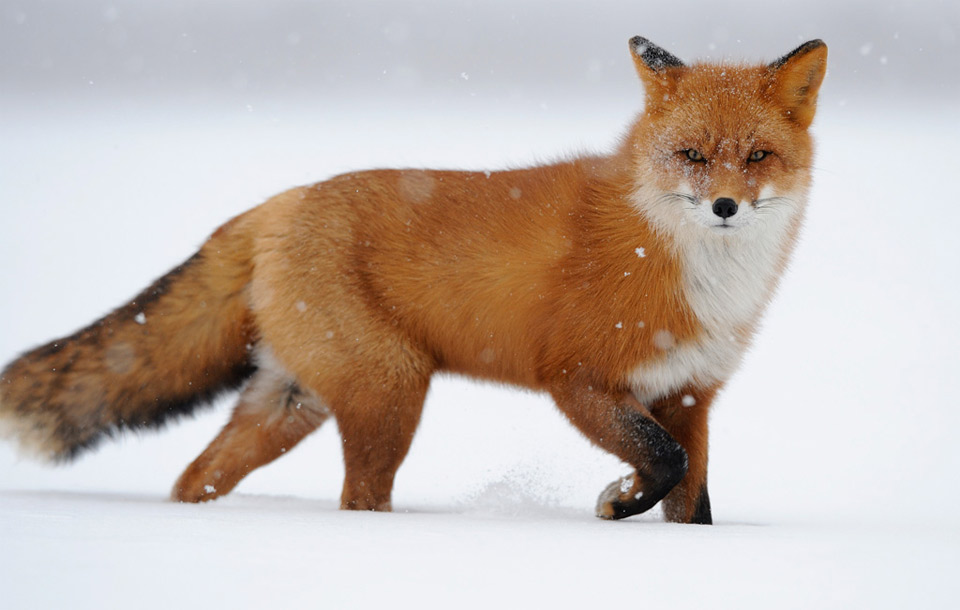
\includegraphics[height=2cm,width=2.5cm]{img/fox.jpg}} $\rightarrow \textrm{``fox''} \rightarrow [2.5, 4.7, 1.006, 0.75, ...]$
        \end{center}
      }
    \end{frame}


    %%%%%%%%%%%%%%%%%%%%%%%%%%%%%%%%%%%%%%%%%%%%%%%%%%%%%%%%%%%%%%%%%%
    %%% Motivation
    \section{Motivation}
    \begin{frame}{\insertsection}
      - What do we need the word embeddings for?
      \begin{example}
        \alt<1,4->{I\_{\tiny SRC} like\_{\tiny SNT} this\_{\tiny NON} car\_{\tiny TRG}}{10\_{\tiny SRC} 178\_{\tiny SNT} 35\_{\tiny NON} 56\_{\tiny TRG}}
      \end{example}

      \begin{example}
        \alt<1,4->{I\_{\tiny NON} drive\_{\tiny NON} this\_{\tiny NON} car\_{\tiny NON}}{10\_{\tiny NON} 208\_{\tiny NON} 35\_{\tiny NON} 56\_{\tiny NON}}
      \end{example}

      \visible<3->{
      \begin{example}
        \only<3>{10\_{\tiny ???} 193\_{\tiny ???} 35\_{\tiny ???} 56\_{\tiny ???}}
        \only<4->{I\_{\tiny ???} love\_{\tiny ???} this\_{\tiny ???} car\_{\tiny ???}}
      \end{example}
      }
    \end{frame}

    \begin{frame}{\insertsection}
      - What do we need word embeddings for?

      - For efficient encoding of lexical information as features.
    \end{frame}

    \begin{frame}{Linguistic Digression}
      - What are word meanings?

      \begin{definition}
        \textbf{Sememe} is the lexical meaning of a word or single morpheme,
        that is commonly understood as a set of semes.\cite{Bussmann:02}
      \end{definition}

      \begin{definition}
        \textbf{Seme} is the smallest unit of meaning recognized in semantics,
        which usually describes one particular property of the pertaining
        object.\cite{Wiki:Seme}
      \end{definition}
    \end{frame}

    \begin{frame}{Linguistic Digression}
      Sememes:\\
      \begin{center}
        \begin{tikzpicture}
          [auto=right,scale=0.6,
            every node/.style={rectangle,draw=none,text width=2cm,font=\tiny,fill=none},
            word/.style={draw=none,fill=none}]

          \node[draw,align=center,text=white,fill=dodgerblue4] (string) at (6,6) {``fox''};

          \node(fox0) at (0,3) {a small wild animal that is related to
            dogs and that has a long pointed nose and a bushy tail};

          \node(fox0pic) at (0,0) {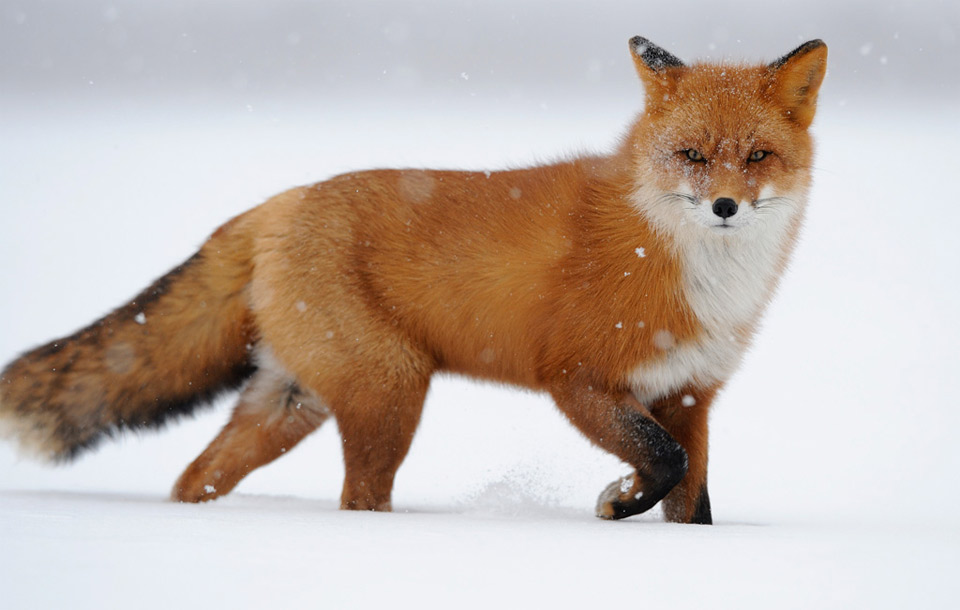
\includegraphics[height=1.5cm,width=2cm]{img/fox.jpg}};

          \node(fox1) at (4,3) {a clever crafty person};

          \node(fox1pic) at (4,0) {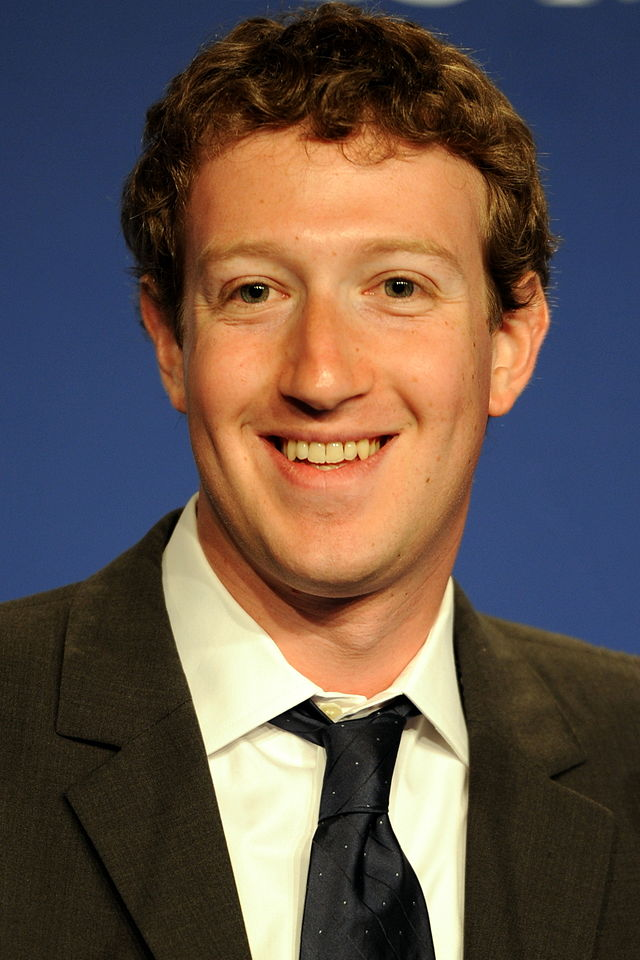
\includegraphics[height=2cm,width=1.5cm]{img/zuckerberg.jpg}};

          \node(fox2) at (8,3) {a good-looking young woman or man};

          \node(fox2pic) at (8,0) {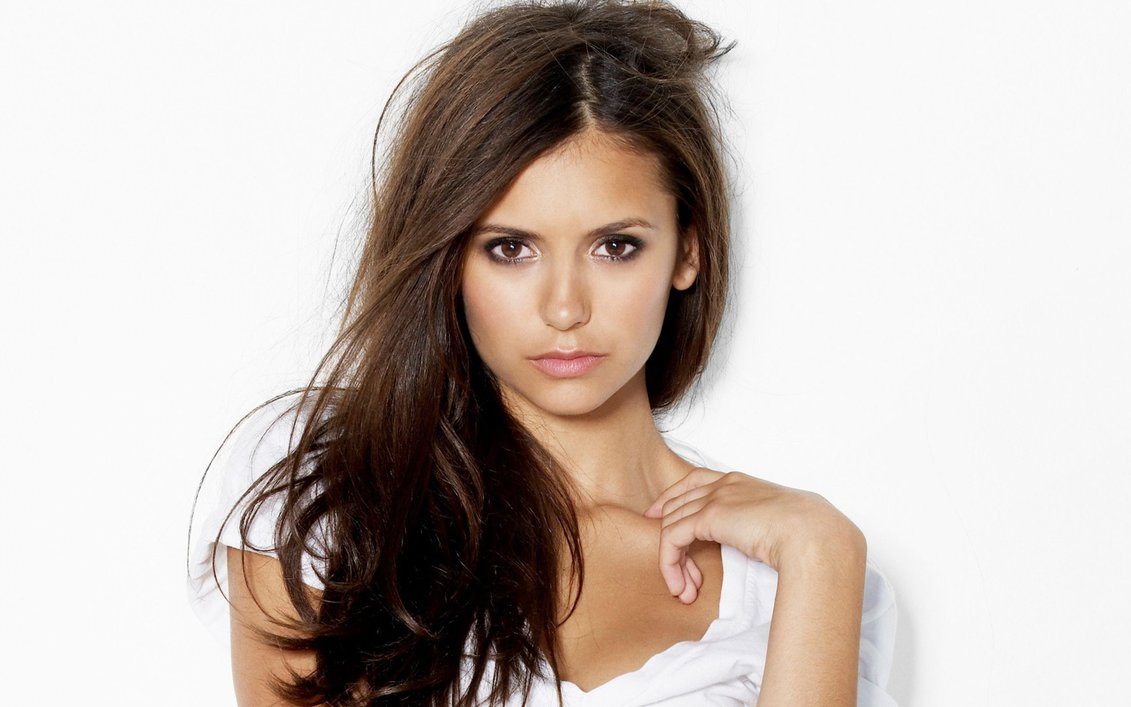
\includegraphics[height=1.5cm,width=1.8cm]{img/model.jpg}};

          \node(fox3) at (12,3) {a member of an American Indian people
            formerly living in what is now Wisconsin};

          \node(fox3pic) at (12,0) {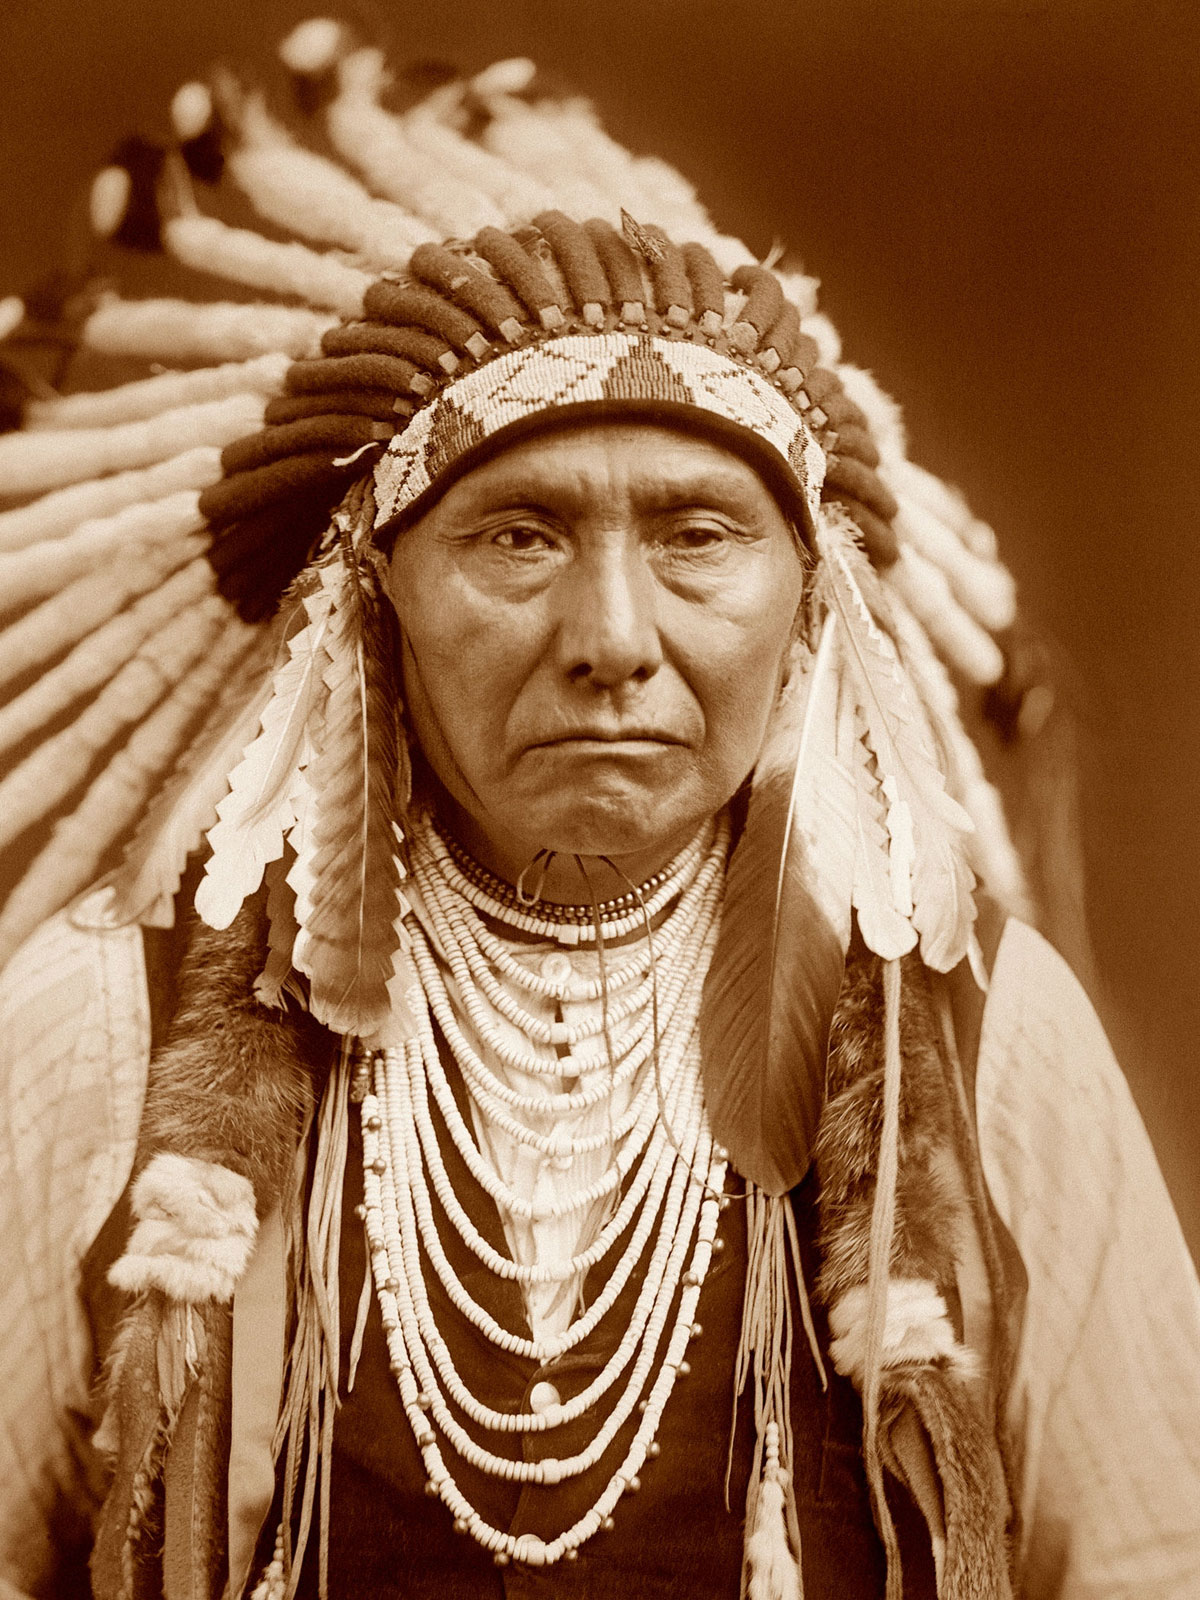
\includegraphics[height=2cm,width=1.5cm]{img/indian.jpg}};

          \foreach \from/\to in {string/fox0,string/fox1,string/fox2,string/fox3}
          \draw (\from) -- (\to);
        \end{tikzpicture}
      \end{center}
    \end{frame}


    \begin{frame}{Linguistic Digression}
      Semes:

      \begin{minipage}[t]{0.25\linewidth}
        \raisebox{-1cm}{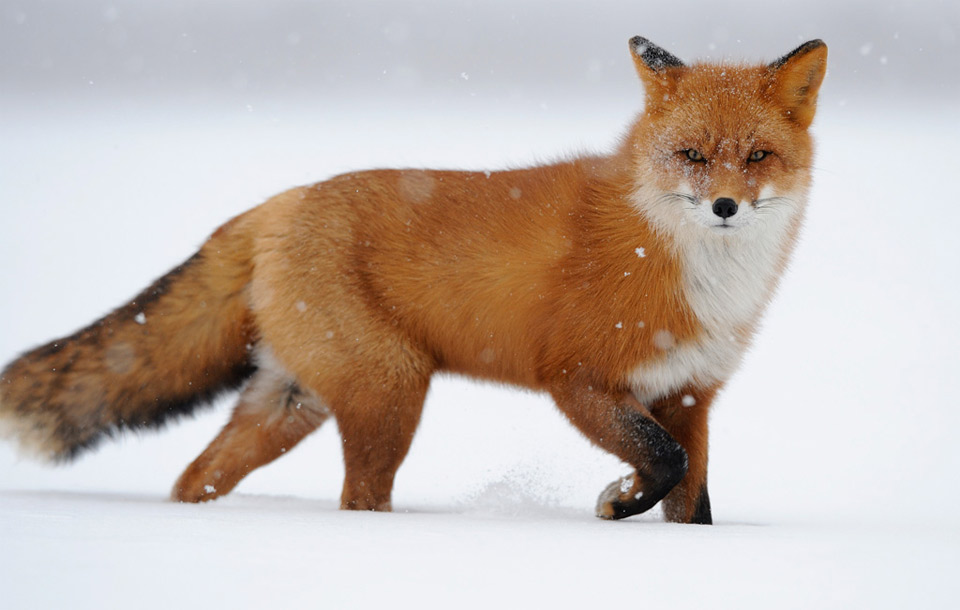
\includegraphics[height=1.5cm,width=2cm]{img/fox.jpg}}%
      \end{minipage}%
      \begin{minipage}[t]{0.70\linewidth}%
        Fox - a small wild animal that is related to dogs and that has a long
        pointed nose and a bushy tail.
      \end{minipage}
      \vfill
      \begin{minipage}[t]{0.45\linewidth}\scriptsize
        \begin{enumerate}
        \item creature (1);
        \item carnivorian (1);
        \item mammal (1);
        \item wild (0.9);
        \item furred (1);
        \item tailed (1);
        \item red-colored (0.9);
        \item four-legged (1);
        \item \dots;%
        \end{enumerate}%
      \end{minipage}\hfill%
      \begin{minipage}[t]{0.45\linewidth}%
        \visible<2->{
          \raisebox{-4cm}{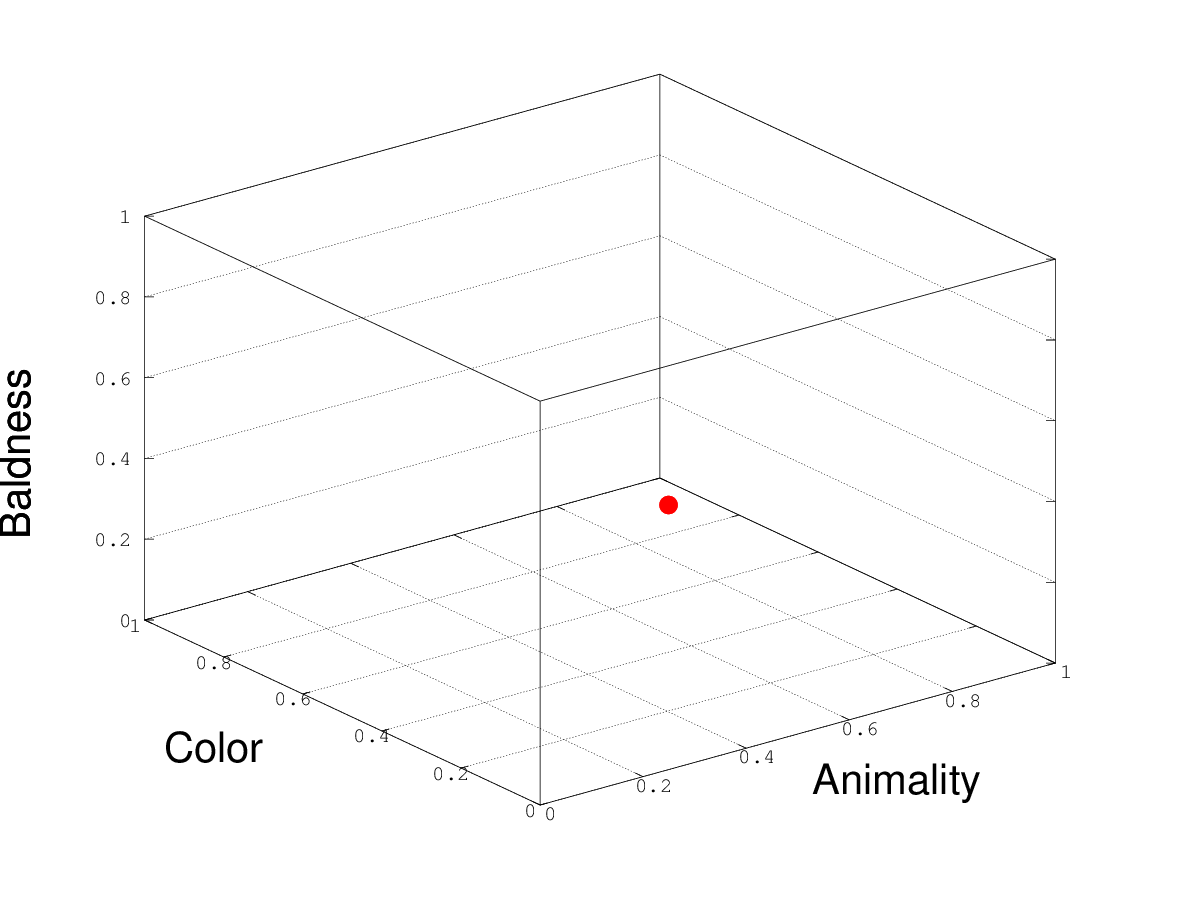
\includegraphics[height=4cm,width=4cm]{img/meaning.png}}
        }
      \end{minipage}
    \end{frame}

    \begin{frame}{Linguistic Digression}
      - What would be the best way to represent word meanings?

      \visible<2->{- Real-valued coordinate vectors $\mathbb{R}^\mathrm{n}$}
    \end{frame}

    \begin{frame}{Linguistic Digression}
      - How do we obtain this ``most natural representation'' automatically?

      \textbf{First attempt}: counter models

      \only<1>{
        \begin{itemize}
        \item counter vectors;
        \item PMI vectors;
        \item PPMI vectors;
        \item factorized counter matrices.
        \end{itemize}
      }

      \textbf{Basic assumption}: words that co-occur together
        should share same or at least compatible semes.

        \only<2->{
          \begin{example}
            The fox ate the hare.
          \end{example}

          \begin{example}
            \alert{The car ate the hare.}
          \end{example}
        }

      \only<3->{\textbf{Main conclusion}: word's co-occurrences already
        are the respective semes of its meaning.}
    \end{frame}

    \begin{frame}{Linguistic Digression}
      - How do we obtain this ``most natural representation'' automatically?

      \textbf{Second attempt}: neural embeddings

      \only<1>{
        \begin{itemize}
          \item \texttt{word2vec};
          \item \texttt{GloVe}.
        \end{itemize}
      }

      \textbf{Basic assumption}: words that co-occur together should share
      same or compatible semes.

      \only<3->{\textbf{Main conclusion}: a word has an inherent latent
        semantic structure and this structure determines its co-occurrence
        with other words.}
    \end{frame}

    \section{Implementation}
    \begin{frame}{Neural Network Digression}
      Neural networks:

      \begin{minipage}[t]{0.5\linewidth}
        \begin{center}
          \vfill{}
          %% \tikzset{mynode1/.style={}}
          %% \tikzset{mynode2/.style={}}
          %% \tikzset{mynode3/.style={}}
          %% \tikzset{mynode4/.style={}}
          %% \tikzset{mynode5/.style={}}
          %% \tikzset{mynode6/.style={}}
          %% \tikzset{mynode7/.style={}}
          %% \tikzset{mynode8/.style={}}
          %% \only<4->{\tikzset{mynode1/.style={text=white,fill=dodgerblue4}}}
          %% \only<5,9,11,12>{\tikzset{mynode2/.style={text=white,fill=dodgerblue4}}}
          %% \only<6,9,11>{\tikzset{mynode3/.style={text=white,fill=dodgerblue4}}}
          %% \only<7,9,11>{\tikzset{mynode4/.style={text=white,fill=dodgerblue4}}}
          %% \only<8,9,11>{\tikzset{mynode5/.style={text=white,fill=dodgerblue4}}}
          %% \only<10,11>{\tikzset{mynode6/.style={text=white,fill=dodgerblue4}}}
          %% \only<12>{\tikzset{mynode7/.style={text=white,fill=dodgerblue4}}}
          %% \only<10,11,12>{\tikzset{mynode8/.style={text=white,fill=dodgerblue4}}}

          %% \tikzset{myedge2/.style={color=white}}
          %% \tikzset{myedge3/.style={color=white}}
          %% \tikzset{myedge4/.style={color=white}}
          %% \tikzset{myedge5/.style={color=white}}
          %% \tikzset{myedge6/.style={color=white}}
          %% \tikzset{myedge7/.style={color=white}}
          %% \only<5,9,11,12>{\tikzset{myedge2/.style={color=black}}}
          %% \only<6,9,11>{\tikzset{myedge3/.style={color=black}}}
          %% \only<7,9,11>{\tikzset{myedge4/.style={color=black}}}
          %% \only<8,9,11>{\tikzset{myedge5/.style={color=black}}}
          %% \only<10,11>{\tikzset{myedge6/.style={color=black}}}
          %% \only<12>{\tikzset{myedge7/.style={color=black}}}
          \begin{tikzpicture}
            [auto=left,scale=0.6,->,
              every node/.style={circle,draw,font=\tiny,fill=gray84,minimum size=15pt},
            ]

            \matrix (m) [matrix of math nodes,ampersand replacement=\&,fill=none,draw=none,rectangle,row sep=0.1cm,%
              column sep=0.8cm] {
              \node[]{}; \& \node[]{};\\
              \node[]{}; \& \node[]{};\\
              \node[]{}; \& \node[]{};\\
              \node[]{}; \& \node[]{};\\
            };

            \foreach \from in {m-1-1,m-2-1,m-3-1,m-4-1}{
              \foreach \to in {m-1-2,m-2-2,m-3-2,m-4-2} {
                \draw (\from) -- (\to);
              };
            };
          \end{tikzpicture}
        \end{center}
        \vfill{}
      \end{minipage}
      \begin{minipage}[t]{0.48\linewidth}
        \scriptsize
        \only<1>{
          Are defined by:
          \begin{itemize}
          \item The number of layers: $L$;
          \item The number of neurons for each layer $l$: $s_l$;
          \item The transition matrices between the layers $l-1$ and $l$:
            $\Theta^{l}_{l-1}$ ($s_{l-1} \times s_l$);
          \item The activation functions $f_l$ which might be specific for
            each layer $l$;
          \item Finally, the cost function: $J_\Theta$.
          \end{itemize}
        }

        \only<2> {
          Objectives of the training:

          Given a set of training instances ${(x_1, y_1), (x_2, y_2), \ldots,
            (x_m, y_m)}$ (where $x \in \mathbb{R}^{s_0}$ and $y \in
          \mathbb{R}^{K}$ so that $K$ is the number of classes), you should
          minimize the cost function $J_\Theta$.\\[0.2cm]
        }

        \only<3> {
          For this, we need to compute:
          \begin{itemize}
            \item The cost function:
              $J_\Theta =
            -\frac{1}{m}\Big[\sum_{i=1}^{m}\sum_{k=1}^{K}y_k^{(i)}log(h_\Theta(x^(i)_k)
              + (1 - y_k^{(i)})log(h_\Theta(x^(i)_k)\Big]$

            \item Partial derivatives with respect to each parameter:
              $\frac{\partial}{\partial \Theta^{(l)}_{ij}} J_\Theta =
              x^{(l)}_i * \delta_j^{(l+1)}$, where $\delta^l = x^l - y$ if $l
              := L$ and $\delta^l = (\Theta^{(l)})^T\delta^{(l + 1)} .*
              f\prime(x^{(l)})$.
          \end{itemize}
        }
      \end{minipage}
      \vspace*{\fill}
    \end{frame}

    \begin{frame}
      \vfill \center At this point, you can lean back and relax.  Because you
      already know almost everything about neural word embeddings, even if
      some of you might not believe that.

      
\includegraphics[height=4cm,width=4cm]{img/relax.jpg}
      \vfill
    \end{frame}

    \begin{frame}{Neural Network Digression}
      Neural networks:

      \begin{minipage}[t]{0.5\linewidth}
        \begin{center}
          \vfill{}
          %% \tikzset{mynode1/.style={}}
          %% \tikzset{mynode2/.style={}}
          %% \tikzset{mynode3/.style={}}
          %% \tikzset{mynode4/.style={}}
          %% \tikzset{mynode5/.style={}}
          %% \tikzset{mynode6/.style={}}
          %% \tikzset{mynode7/.style={}}
          %% \tikzset{mynode8/.style={}}
          %% \only<4->{\tikzset{mynode1/.style={text=white,fill=dodgerblue4}}}
          %% \only<5,9,11,12>{\tikzset{mynode2/.style={text=white,fill=dodgerblue4}}}
          %% \only<6,9,11>{\tikzset{mynode3/.style={text=white,fill=dodgerblue4}}}
          %% \only<7,9,11>{\tikzset{mynode4/.style={text=white,fill=dodgerblue4}}}
          %% \only<8,9,11>{\tikzset{mynode5/.style={text=white,fill=dodgerblue4}}}
          %% \only<10,11>{\tikzset{mynode6/.style={text=white,fill=dodgerblue4}}}
          %% \only<12>{\tikzset{mynode7/.style={text=white,fill=dodgerblue4}}}
          %% \only<10,11,12>{\tikzset{mynode8/.style={text=white,fill=dodgerblue4}}}

          %% \tikzset{myedge2/.style={color=white}}
          %% \tikzset{myedge3/.style={color=white}}
          %% \tikzset{myedge4/.style={color=white}}
          %% \tikzset{myedge5/.style={color=white}}
          %% \tikzset{myedge6/.style={color=white}}
          %% \tikzset{myedge7/.style={color=white}}
          %% \only<5,9,11,12>{\tikzset{myedge2/.style={color=black}}}
          %% \only<6,9,11>{\tikzset{myedge3/.style={color=black}}}
          %% \only<7,9,11>{\tikzset{myedge4/.style={color=black}}}
          %% \only<8,9,11>{\tikzset{myedge5/.style={color=black}}}
          %% \only<10,11>{\tikzset{myedge6/.style={color=black}}}
          %% \only<12>{\tikzset{myedge7/.style={color=black}}}
          \begin{tikzpicture}
            [auto=left,scale=0.6,->,
              every node/.style={circle,draw,font=\tiny,fill=gray84,minimum size=15pt},
            ]

            \matrix (m) [matrix of math nodes,ampersand replacement=\&,fill=none,draw=none,rectangle,row sep=0.1cm,%
              column sep=0.8cm] {
              \node[]{}; \& \node[]{};\\
              \node[]{}; \& \node[]{};\\
              \node[]{}; \& \node[]{};\\
              \node[]{}; \& \node[]{};\\
            };

            \foreach \from in {m-1-1,m-2-1,m-3-1,m-4-1}{
              \foreach \to in {m-1-2,m-2-2,m-3-2,m-4-2} {
                \draw (\from) -- (\to);
              };
            };
          \end{tikzpicture}
        \end{center}
        \vfill{}
      \end{minipage}
      \begin{minipage}[t]{0.48\linewidth}
        \scriptsize

        As you might remember, neural networks are defined by the following
        components:
        \begin{itemize}
        \item The number of layers: $L$\visible<2->{$= 2$ (the input word and
          the co-occurrence word)};
        \item The number of neurons for each layer $l$: $s_l$ \visible<2->{is
          the same for both layers; it is set manually through a parameter and
          roughly corresponds to the dimensionality of the vector space (or
          the number of semes that you want to encode)};
        \item The transition matrices between the layers $l-1$ and $l$:
          $\Theta^{l}_{l-1}$ ($s_{l-1} \times s_l$) \visible<2->{well, they
          don't exist explicitly in \texttt{word2vec} or we could say that it
          is equal to trhe identity matrix $I$};
        \item The activation functions $f_l$ which might be specific for each
          layer $l$ \visible<2->{yeap, at the output layer you have the
            softmax};
        \item Finally, the cost function: $J_\Theta$.
        \end{itemize}
      \end{minipage}
    \end{frame}

    \section*{Bibliography}
    \bibliography{bibliography}
    \bibliographystyle{plain}
    \end{document}
